% Figure 5.6: Transformer Encoder Architecture
% Compile with: pdflatex fig_5_6_transformer_architecture.tex

\documentclass[border=10pt]{standalone}
\usepackage{tikz}
\usetikzlibrary{shapes.geometric, arrows.meta, positioning}
\usepackage{xcolor}
\usepackage{amsmath}

% Professional academic color palette
\definecolor{inputgray}{RGB}{220, 220, 220}
\definecolor{embedblue}{RGB}{176, 196, 222}    % Light steel blue
\definecolor{attnpurple}{RGB}{186, 175, 201}   % Lavender gray
\definecolor{ffnorange}{RGB}{222, 184, 135}    % Burlywood
\definecolor{normblue}{RGB}{173, 198, 215}     % Light slate blue
\definecolor{outputgreen}{RGB}{176, 208, 176}  % Sage green
\definecolor{textdark}{RGB}{33, 33, 33}
\definecolor{blockbg}{RGB}{250, 250, 250}

\begin{document}
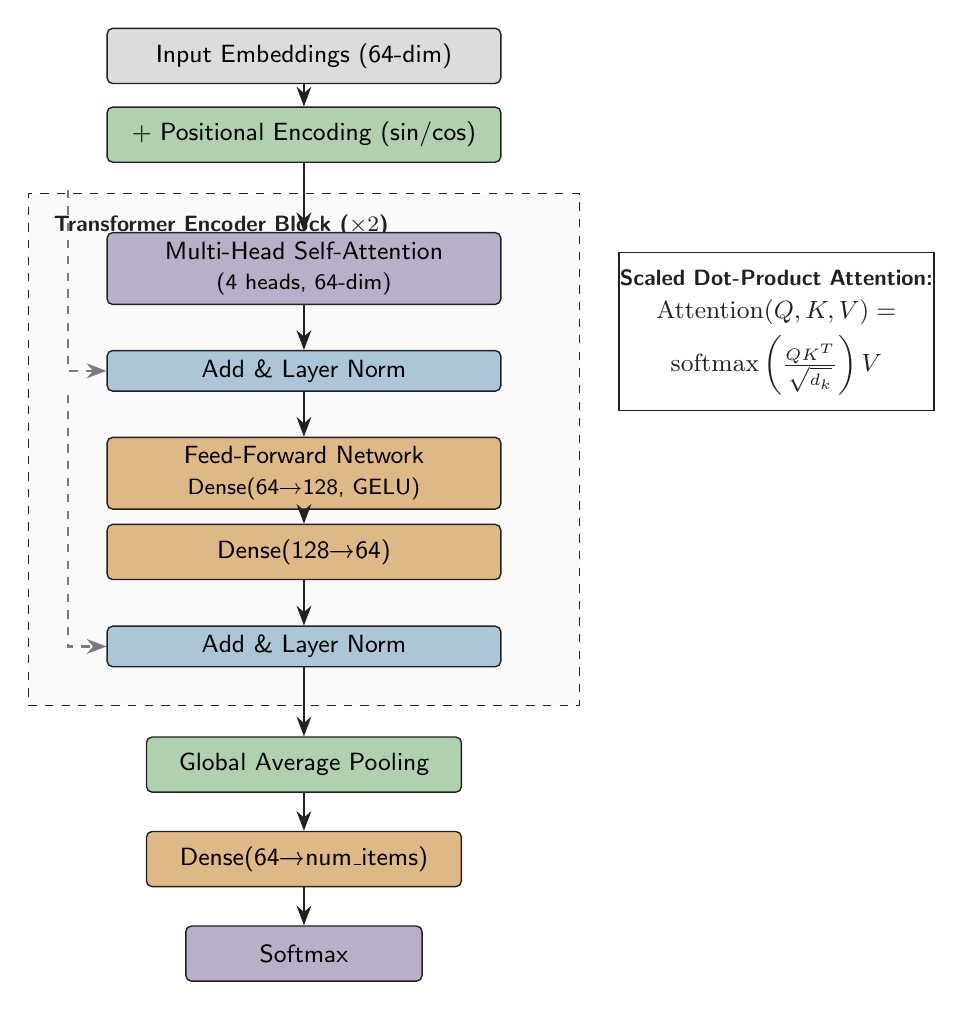
\begin{tikzpicture}[
    node distance=0.8cm,
    layer/.style={rectangle, draw=textdark, rounded corners=2pt, minimum width=3cm, minimum height=0.7cm, align=center, font=\small\sffamily, line width=0.5pt},
    attention/.style={layer, fill=attnpurple},
    ffn/.style={layer, fill=ffnorange},
    norm/.style={layer, fill=normblue, minimum height=0.5cm},
    arrow/.style={-{Stealth[length=2.5mm]}, thick, color=textdark},
]

% Input
\node[layer, fill=inputgray, minimum width=5cm] (input) at (0, 7.5) {Input Embeddings (64-dim)};
\node[layer, fill=outputgreen, minimum width=5cm] (pos) at (0, 6.5) {+ Positional Encoding (sin/cos)};

\draw[arrow] (input) -- (pos);

% Transformer block (repeated)
\node[rectangle, draw=textdark, dashed, fill=blockbg, minimum width=7cm, minimum height=6.5cm, line width=0.5pt] (block) at (0, 2.5) {};
\node[font=\footnotesize\bfseries\sffamily, anchor=north west, color=textdark] at (-3.3, 5.6) {Transformer Encoder Block ($\times 2$)};

% Multi-head attention
\node[attention, minimum width=5cm] (mha) at (0, 4.8) {Multi-Head Self-Attention\\{\footnotesize\sffamily (4 heads, 64-dim)}};

% Add & Norm 1
\node[norm, minimum width=5cm] (norm1) at (0, 3.5) {Add \& Layer Norm};

% FFN
\node[ffn, minimum width=5cm] (ffn1) at (0, 2.2) {Feed-Forward Network\\{\footnotesize\sffamily Dense(64→128, GELU)}};
\node[ffn, minimum width=5cm] (ffn2) at (0, 1.2) {Dense(128→64)};

% Add & Norm 2
\node[norm, minimum width=5cm] (norm2) at (0, 0) {Add \& Layer Norm};

% Residual connections
\draw[arrow] (pos) -- (mha);
\draw[arrow] (mha) -- (norm1);
\draw[arrow] (norm1) -- (ffn1);
\draw[arrow] (ffn1) -- (ffn2);
\draw[arrow] (ffn2) -- (norm2);

% Residual arrows
\draw[arrow, dashed, color=textdark!60] (-3, 5.8) -- (-3, 3.5) -- (norm1.west);
\draw[arrow, dashed, color=textdark!60] (-3, 3.2) -- (-3, 0) -- (norm2.west);

% Output layers
\node[layer, fill=outputgreen, minimum width=4cm] (pool) at (0, -1.5) {Global Average Pooling};
\node[layer, fill=ffnorange, minimum width=4cm] (out) at (0, -2.7) {Dense(64→num\_items)};
\node[layer, fill=attnpurple] (softmax) at (0, -3.9) {Softmax};

\draw[arrow] (norm2) -- (pool);
\draw[arrow] (pool) -- (out);
\draw[arrow] (out) -- (softmax);

% Attention detail
\node[rectangle, draw=textdark, minimum width=4cm, minimum height=2cm, line width=0.5pt] (attndetail) at (6, 4) {};
\node[font=\footnotesize\bfseries\sffamily, anchor=north, color=textdark] at (6, 4.9) {Scaled Dot-Product Attention:};
\node[font=\small, align=center, color=textdark] at (6, 3.8) {$\text{Attention}(Q,K,V) =$\\[3pt]$\text{softmax}\left(\frac{QK^T}{\sqrt{d_k}}\right)V$};

\end{tikzpicture}
\end{document}
